\begin{center}
	\section{Sedimentaci\'on}
\end{center}

\noindent
\justify

El \textit{principio funcional} del sistema de eluci\'on y filtrado de la planta de extracci\'on recae en este fen\'omeno natural.

\noindent
\justify

Los tanques de sedimentaci\'on son ampliamente usados como medios filtrantes en plantas purificadoras de agua debido a su capacidad de remoci\'on de residuos s\'olidos; siendo empleadas para limpiar aguas con turbidez\footnote{La turbidez define el nivel de transparencia de fluidos incoloros en contraste a la presencia de part\'iculas en suspensi\'on.} de hasta $50 [NTU]^{\cite{Voutchkov2017}}$\footnote{La Organizaci\'on Mundial de la Salud estipula que el agua de consumo humano debe presentar un nivel de turbidez inferior a $2 [NTU]^{\cite{OMSagua}}$.}. 

\noindent
\justify

Para asegurar un correcto nivel de turbidez, los sistemas de sedimentaci\'on convencionales emplean coagulantes (normalmente sales de hierro) y floculantes (pol\'imeros) en el sistema de alimentaci\'on. Cuando el fluido excede el nivel de $50 [NTU]$, se recomienda emplear sistemas de sedimentaci\'on de placas inclinadas$^{\cite{Voutchkov2017}}$ para la remoci\'on de elementos s\'olidos de bajo tama\~no de part\'icula.


\subsection{Sedimentadores convencionales}

\noindent
\justify

Son ampliamente usados para la remoci\'on de part\'iculas en fluidos con turbidez de $20 [NTU]^{\cite{Voutchkov2017}}$. Consiste de un sistema de una sola etapa estructurado de forma circular o rectangular. A la fecha, sedimentadores rectangulares se emplean sistemas de pretratamiento de aguas salinas por su bajo costo de inversi\'on y gran desempe\~no. Los par\'ametros clave para el dise\~no de estos sistemas son los siguientes:

\begin{itemize}
	\item N\'umero m\'inimo de tanques: 4
	\item Produndidad del agua: $3.0 - 4.0 [m]$.
	\item Velocidad media de flujo: $0.3 - 1.1 [m/min]$.
	\item Tiempo de detenci\'on: $2 - 4 [h]$.
	\item Relaci\'on ancho-largo: m\'inimo de 4:1.
	\item Relaci\'on profundidad-largo: m\'inimo de 1:15 
	\item Velocidad del recolector de lodos: $0.4 - 0.8 [m/min]$.
\end{itemize}

\newpage

\subsection{Sedimentador de placas inclinadas}

\noindent
\justify

Estos tanques de sedimentaci\'on, tambi\'en conocidos como \textit{clarificadores}, tienen un desempe\~no altamente superior a los convencionales, llegando a clarificar fluidos de hasta $200 [NTU]^{\cite{Voutchkov2017}}$ de turbidez. Normalmente tienen una estructura rectangular o circular y son ampliamente usados para la limpieza de agua marina. 

\begin{figure}[h!]
	\centering
	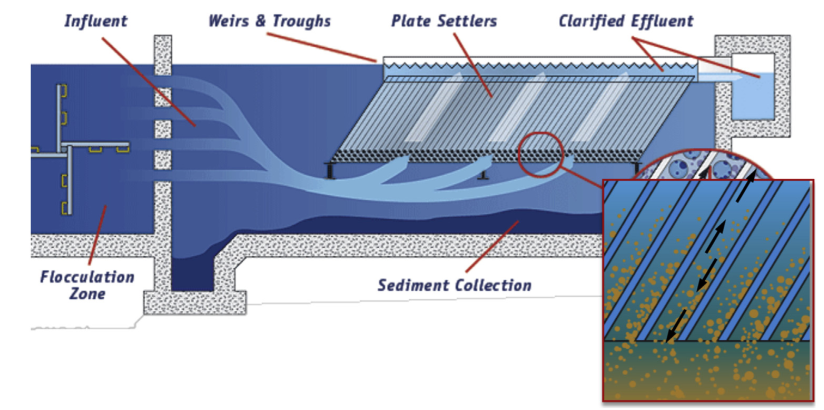
\includegraphics[width=\textwidth]{Images/lamelas_inclinadas.png}
	\caption{Esquema de un sedimentador de placas inclinadas$^{\cite{Voutchkov2017}}$.}
	\label{lamelas_inclinadas}
\end{figure}


\noindent
\justify

Los criterios clave de dise\~no para su uso en plantas de trateminto de agua se evidencia a continuaci\'on:

\begin{itemize}
	\item N\'umero m\'inimo de tanques: 2
	\item Produndidad del agua: $3.5 - 5.0 [m]$.
	\item Velocidad media de flujo: $0.3 - 1.1 [m/min]$.
	\item Tiempo de detenci\'on: $0.2 - 0.4 [h]$.
	\item Velocidad del recolector de lodos: $0.4 - 0.8 [m/min]$.
\end{itemize}

\subsubsection{Desarrollo te\'orico}

\noindent
\justify

